\documentclass{slides}
\usepackage[latin1]{inputenc}
\usepackage{fancyvrb}
\usepackage{ngerman}
\usepackage{epsfig}
\usepackage{amssymb}
%\usepackage{pstricks,pstcol,pst-node} % comment this to make xdvi work

\pagestyle{empty}
\setlength{\textwidth}{17cm}
\setlength{\textheight}{24cm}
\setlength{\topmargin}{0cm}
\setlength{\headheight}{0cm}
\setlength{\headsep}{0cm}
\setlength{\topskip}{0.2cm}
\setlength{\oddsidemargin}{0.5cm}
\setlength{\evensidemargin}{0.5cm}

\newcommand{\squoted}[1]{\mbox{``\texttt{#1}''}}
\newcommand{\quoted}[1]{\;\mbox{``\texttt{#1}''}\;}
\newcommand{\schluss}[2]{\frac{\displaystyle\quad \rule[-6pt]{0pt}{12pt}#1 \quad}{\displaystyle\quad \rule{0pt}{10pt}#2 \quad}}
\newcommand{\mathquote}[1]{\mbox{``}\mathtt{#1}\mbox{''}}
\newcommand{\bruch}[2]{\frac{\displaystyle#1}{\displaystyle #2}}

\newcounter{mypage}

\begin{document}

\begin{slide}{}
\normalsize
\begin{center}
\"Uberblick \"uber die Vorlesung
\end{center}
\vspace{0.5cm}

\footnotesize
\begin{enumerate}
\item Definition: Formale Sprachen
\item Regul\"are Ausdr\"ucke: Spezifikation von Strings

      wichtig in Skriptsprachen
 
      \textsl{Tcl}, \textsl{Perl}, \textsl{Python}, \textsl{Ruby}, $\cdots$
\item Anwendungen regul\"arer Ausdr\"ucke

      \texttt{flex}: \emph{\underline{f}ast \underline{lex}ical analyser generator}.

      \emph{Scanner-Generator}
\item Endliche Automaten
      
\item Kontextfreie Sprachen

\item \textsc{Antlr}, \textsl{Bison}: Parser-Generatoren

\item Keller-Automaten

\item Theorie der LL(k)-Sprachen

      Grundlage von \textsc{Antlr}
\end{enumerate}

\vspace*{\fill}
\tiny \addtocounter{mypage}{1}
\rule{17cm}{1mm}
\"Uberblick  \hspace*{\fill} Seite \arabic{mypage}
\end{slide}

%%%%%%%%%%%%%%%%%%%%%%%%%%%%%%%%%%%%%%%%%%%%%%%%%%%%%%%%%%%%%%%%%%%%%%%%

\begin{slide}{}
\normalsize
\begin{center}
\"Uberblick, Teil \texttt{II}
\end{center}
\vspace{0.5cm}

\footnotesize
\begin{enumerate}
\item Theorie der LL($*$)-Sprachen (\textsc{Antlr})

\item Grenzen kontextfreier Sprachen

\item Interpreter

\item Theorie der LALR-Sprachen

      Grundlage von \textsl{Bison}
\item Der Parser-Generator \textsl{JavaCup}

      \textsl{JavaCup} ist ein LALR-Parser-Generator f\"ur \textsl{Java}.
\item Typ-\"Uberpr\"ufung
  
\item Entwicklung eines einfacher Compiler
\item Register-Zuordnung  
\end{enumerate}

\vspace*{\fill}
\tiny \addtocounter{mypage}{1}
\rule{17cm}{1mm}
\"Uberblick  \hspace*{\fill} Seite \arabic{mypage}
\end{slide}

%%%%%%%%%%%%%%%%%%%%%%%%%%%%%%%%%%%%%%%%%%%%%%%%%%%%%%%%%%%%%%%%%%%%%%%%

\begin{slide}{}
\normalsize
\begin{center}
Literatur
\end{center}
\vspace{0.5cm}

\footnotesize
\begin{enumerate}
\item Skript
\item \emph{Introduction to Automata Theory, Languages, and Computation}

      John E. Hopcroft, Rajeev Motwani, Jeffrey D. Ullman
\item \emph{lex \& yacc} 

      John R. Levine, Tony Mason, Doug Brown
\item \emph{Compilers --- Principles, Techniques and Tools}

      Alfred V. Aho, Ravi Sethi, Jeffrey D. Ullman, \\
      Monica S. Lam
\item \emph{Mastering Regular Expressions}

      Jeffrey E. F. Friedl
\end{enumerate}

\vspace*{\fill}
\tiny \addtocounter{mypage}{1}
\rule{17cm}{1mm}
Literatur  \hspace*{\fill} Seite \arabic{mypage}
\end{slide}



%%%%%%%%%%%%%%%%%%%%%%%%%%%%%%%%%%%%%%%%%%%%%%%%%%%%%%%%%%%%%%%%%%%%%%%%

\begin{slide}{}
\normalsize
\begin{center}
Algebra regul\"arer Ausdr\"ucke
\end{center}
\vspace{0.5cm}

\footnotesize

\begin{enumerate}
\item $r_1 + r_2 \doteq r_2 + r_1$
\item $(r_1 + r_2) + r_3 \doteq r_1 + (r_2 + r_3)$
\item $(r_1 \cdot r_2) \cdot r_3 \doteq r_1 \cdot (r_2 \cdot r_3)$
\item $\emptyset \cdot r \doteq r \cdot \emptyset \doteq \emptyset$
\item $\varepsilon \cdot r \doteq r \cdot \varepsilon \doteq r$
\item $\emptyset + r \doteq r + \emptyset \doteq r$
\item $(r_1 + r_2) \cdot r_3 \doteq r_1 \cdot r_3 + r_2 \cdot r_3$
\item $r_1 \cdot (r_2 + r_3) \doteq r_1 \cdot r_2 + r_1 \cdot r_3$
\item $r + r \doteq r$
\item $(r^*)^* \doteq r^*$      
\item $\emptyset^* \doteq \varepsilon$
\item $\varepsilon^* \doteq \varepsilon$
\item $r^* \doteq \varepsilon + r^* \cdot r$
\item $r^* \doteq (\varepsilon + r)^*$
\end{enumerate}
Schluss-Regel:\quad
$\bruch{r \doteq r \cdot s + t \quad \varepsilon \not\in L(s)}{r \doteq t \cdot s^*}$


\vspace*{\fill}
\tiny \addtocounter{mypage}{1}
\rule{17cm}{1mm}
algebraische Vereinfachungen  \hspace*{\fill} Seite \arabic{mypage}
\end{slide}

%%%%%%%%%%%%%%%%%%%%%%%%%%%%%%%%%%%%%%%%%%%%%%%%%%%%%%%%%%%%%%%%%%%%%%%%%

%\begin{slide}{}
%\normalsize
%\begin{center}
%Deterministische und nicht-deterministische endliche Automaten
%\end{center}
%\vspace{0.5cm}

%\footnotesize


% \begin{pspicture}(-1,-1)(11.000000,10.000000)
% %%\newpsobject{showgrid}{psgrid}{subgriddiv=1,griddots=10,gridlabels=6pt}
% %%\showgrid
% \psset{unit=0.025cm}
%\rput(0.000000,180.000000){\circlenode[]{0}{$q_0$}}
%\pnode(-40.000000,180.000000){start0}
%\ncarc[arcangle=0]{->}{start0}{0}
%\rput(120.000000,180.000000){\circlenode[]{7}{$q_7$}}
%\rput(240.000000,300.000000){\circlenode[]{5}{$q_5$}}
%\rput(360.000000,360.000000){\circlenode[doubleline=true]{3}{$q_3$}}
%\rput(360.000000,240.000000){\circlenode[doubleline=true]{4}{$q_4$}}
%\rput(240.000000,60.000000){\circlenode[]{6}{$q_6$}}
%\rput(360.000000,120.000000){\circlenode[doubleline=true]{1}{$q_1$}}
%\rput(360.000000,0.000000){\circlenode[doubleline=true]{2}{$q_2$}}

%%transition from 0 to 0 with a
%\nccircle[angle=0]{<-}{0}{0.5cm}
%\nbput{\rnode{x}{a}}

%%transition from 0 to 7 with b
%\ncarc[arcangle=15.000000]{->}{0}{7}
%\naput{\rnode{x}{b}}

%%transition from 7 to 5 with a
%\ncarc[arcangle=15.000000]{->}{7}{5}
%\naput{\rnode{x}{a}}

%%transition from 7 to 6 with b
%\ncarc[arcangle=15.000000]{->}{7}{6}
%\naput{\rnode{x}{b}}

%%transition from 5 to 3 with b
%\ncarc[arcangle=15.000000]{->}{5}{3}
%\naput{\rnode{x}{b}}

%%transition from 5 to 4 with a
%\ncarc[arcangle=15.000000]{->}{5}{4}
%\naput{\rnode{x}{a}}

%%transition from 3 to 5 with a
%\ncarc[arcangle=15.000000]{->}{3}{5}
%\naput{\rnode{x}{a}}

%%transition from 3 to 6 with b
%\ncarc[arcangle=15.000000]{->}{3}{6}
%\naput{\rnode{x}{b}}

%%transition from 4 to 0 with a
%\ncarc[arcangle=15.000000]{->}{4}{0}
%\naput{\rnode{x}{a}}

%%transition from 4 to 7 with b
%\ncarc[arcangle=15.000000]{->}{4}{7}
%\naput{\rnode{x}{b}}

%%transition from 6 to 1 with b
%\ncarc[arcangle=15.000000]{->}{6}{1}
%\naput{\rnode{x}{b}}

%%transition from 6 to 2 with a
%\ncarc[arcangle=15.000000]{->}{6}{2}
%\naput{\rnode{x}{a}}

%%transition from 1 to 1 with b
%\nccircle[angle=-90]{<-}{1}{0.5cm}
%\trput{\rnode{x}{b}}

%%transition from 1 to 2 with a
%\ncarc[arcangle=15.000000]{->}{1}{2}
%\naput{\rnode{x}{a}}

%%transition from 2 to 3 with b
%\ncarc[arcangle=15.000000]{->}{2}{3}
%\naput{\rnode{x}{b}}

%%transition from 2 to 4 with a
%\ncarc[arcangle=15.000000]{->}{2}{4}
%\naput{\rnode{x}{a}}
%\end{pspicture}


% \begin{pspicture}(-1,0)(10,3)
% %% \newpsobject{showgrid}{psgrid}{subgriddiv=1,griddots=10,gridlabels=6pt}
% %% \showgrid
% \psset{unit=0.025cm}
%\rput(0.000000,40){\circlenode[]{0}{$q_0$}}
%\pnode(-40.000000,40){start0}
%\ncarc[arcangle=0]{->}{start0}{0}
%\rput(120,40){\circlenode[]{1}{$q_1$}}
%\rput(240,40){\circlenode[]{2}{$q_2$}}
%\rput(360,40){\circlenode[doubleline=true]{3}{$q_3$}}

%%transition from 0 to 0 with a, b
%\nccircle[angle=0]{<-}{0}{0.5cm}
%\nbput{\rnode{x}{a,b}}

%%transition from 0 to 1 with b
%\ncarc[arcangle=15]{->}{0}{1}
%\naput{\rnode{x}{b}}

%%transition from 1 to 2 with a, b
%\ncarc[arcangle=15]{->}{1}{2}
%\naput{\rnode{x}{a,b}}

%%transition from 2 to 3 with a, b
%\ncarc[arcangle=15]{->}{2}{3}
%\naput{\rnode{x}{a,b}}

%\end{pspicture}

% \begin{pspicture}(-1,0)(14,5)
% %% \newpsobject{showgrid}{psgrid}{subgriddiv=1,griddots=10,gridlabels=6pt}
% %% \showgrid
% \psset{unit=0.025cm}
%\rput(0.000000,100){\circlenode[]{0}{$q_0$}}
%\pnode(-40.000000,100){start0}
%\ncarc[arcangle=0]{->}{start0}{0}
%\rput(120,150){\circlenode[]{1}{$q_1$}}
%\rput(240,150){\circlenode[]{3}{$q_3$}}
%\rput(360,150){\circlenode[]{5}{$q_5$}}
%\rput(120, 50){\circlenode[]{2}{$q_2$}}
%\rput(240, 50){\circlenode[]{4}{$q_4$}}
%\rput(360, 50){\circlenode[]{6}{$q_6$}}
%\rput(480,100){\circlenode[doubleline=true]{7}{$q_7$}}

%%transition from 0 to 1 with epsilon
%\ncarc[arcangle=0]{->}{0}{1}
%\naput{\rnode{x}{$\varepsilon$}}

%%transition from 1 to 3 with b
%\ncarc[arcangle=0]{->}{1}{3}
%\naput{\rnode{x}{b}}

%%transition from 3 to 5 with a
%\ncarc[arcangle=0]{->}{3}{5}
%\naput{\rnode{x}{a}}

%%transition from 5 to 7 with epsilon
%\ncarc[arcangle=0]{->}{5}{7}
%\naput{\rnode{x}{$\varepsilon$}}

%%transition from 0 to 2 with epsilon
%\ncarc[arcangle=-0]{->}{0}{2}
%\nbput{\rnode{x}{$\varepsilon$}}

%%transition from 2 to 4 with a
%\ncarc[arcangle=-0]{->}{2}{4}
%\nbput{\rnode{x}{a}}

%%transition from 4 to 6 with b
%\ncarc[arcangle=-0]{->}{4}{6}
%\nbput{\rnode{x}{b}}

%%transition from 6 to 7 with epsilon
%\ncarc[arcangle=-0]{->}{6}{7}
%\nbput{\rnode{x}{$\varepsilon$}}

%%transition from 7 to 0 with epsilon
%\ncarc[arcangle=-0]{->}{7}{0}
%\nbput{\rnode{x}{$\varepsilon$}}

%\end{pspicture}



%\vspace*{\fill}
%\tiny \addtocounter{mypage}{1}
%\rule{17cm}{1mm}
%deterministische und nicht-deterministische endliche Automaten  
%\end{slide}

%%%%%%%%%%%%%%%%%%%%%%%%%%%%%%%%%%%%%%%%%%%%%%%%%%%%%%%%%%%%%%%%%%%%%%%%

\begin{slide}{}
\normalsize
\begin{center}
Eine Grammatik f\"ur arithmetische Ausdr\"ucke
\end{center}
\vspace{1.5cm}

\footnotesize

\begin{center}
 
  \framebox{
  \framebox{
  \begin{minipage}[t]{14cm}
  
\begin{eqnarray*}
  \textsl{ArithExpr} & \rightarrow & \textsl{ArithExpr} \quoted{+} \textsl{Product}  \\
                     & \mid        & \textsl{ArithExpr} \quoted{-} \textsl{Product}  \\
                     & \mid        & \textsl{Product} \\[0.2cm]
  \textsl{Product}   & \rightarrow & \textsl{Product} \quoted{*} \textsl{Factor}    \\
                     & \mid        & \textsl{Product} \quoted{/} \textsl{Factor}     \\
                     & \mid        & \textsl{Factor} \\[0.2cm]
  \textsl{Factor}    & \rightarrow & \quoted{(} \textsl{ArithExpr} \quoted{)} \\
                     & \mid        & \texttt{NUMBER}
\end{eqnarray*}
\vspace*{-0.5cm}

  \end{minipage}}}
\end{center}

\vspace*{\fill}
\tiny \addtocounter{mypage}{1}
\rule{17cm}{1mm}
Grammatik f\"ur arithmetische Ausdr\"ucke  \hspace*{\fill} Seite \arabic{mypage}
\end{slide}

%%%%%%%%%%%%%%%%%%%%%%%%%%%%%%%%%%%%%%%%%%%%%%%%%%%%%%%%%%%%%%%%%%%%%%%%

\begin{slide}{}
\normalsize
\begin{center}
Entfernen von Links-Rekursion
\end{center}
\vspace{1.5cm}

\footnotesize

Gegeben: links-rekursive Grammatik f\"ur Variable $A$
\begin{center}
  \framebox{
  \framebox{
  \begin{minipage}[t]{8cm}
$$
\begin{array}[t]{lcl}
A & \rightarrow & A \beta_1 \\
  & \mid        & A \beta_2 \\
  & \vdots      & \vdots    \\
  & \mid        & A \beta_k \\[0.3cm]
  & \mid        & \gamma_1  \\
  & \vdots      & \vdots    \\
  & \mid        & \gamma_l  \\[0.3cm]
\end{array}
$$
\end{minipage}}}
\end{center}

Transformation in nicht-links-rekursive Grammatik
\begin{center}
  \framebox{
  \framebox{
  \begin{minipage}[t]{12cm}
$$
\begin{array}[t]{lcl}
A & \rightarrow & \gamma_1\;L \;\mid\; \gamma_2\;L \;\mid\; \cdots \;\mid\; \gamma_l\;L  \\[0.2cm]
L & \rightarrow & \beta_1 \;L \;\mid\; \beta_2 \;L \;\mid\; \cdots \;\mid\; \beta_k \;L \;\mid\; \varepsilon
\end{array}
$$
\end{minipage}}}
\end{center}

\vspace*{\fill}
\tiny \addtocounter{mypage}{1}
\rule{17cm}{1mm}
Grammatik  ohne Links-Rekursion \hspace*{\fill} Seite \arabic{mypage}
\end{slide}

%%%%%%%%%%%%%%%%%%%%%%%%%%%%%%%%%%%%%%%%%%%%%%%%%%%%%%%%%%%%%%%%%%%%%%%%

\begin{slide}{}
\normalsize
\begin{center}
Eine Grammatik f\"ur arithmetische Ausdr\"ucke ohne Links-Rekursion
\end{center}
\vspace{1.5cm}

\footnotesize
  \begin{center}    
  \framebox{
  \framebox{
  \begin{minipage}[t]{12cm}

  \begin{eqnarray*}
  \textsl{Expr}        & \rightarrow & \;\textsl{Product}\;\;\textsl{ExprRest}            \\[0.2cm]
  \textsl{ExprRest}    & \rightarrow & \quoted{+} \textsl{Product}\;\;\textsl{ExprRest}   \\
                       & \mid        & \quoted{-} \textsl{Product}\;\;\textsl{ExprRest}   \\
                       & \mid        & \;\varepsilon                                      \\[0.2cm]
  \textsl{Product}     & \rightarrow & \;\textsl{Factor}\;\;\textsl{ProdRest}          \\[0.2cm]
  \textsl{ProdRest} & \rightarrow & \quoted{*} \textsl{Factor}\;\;\textsl{ProdRest} \\
                       & \mid        & \quoted{/} \textsl{Factor}\;\;\textsl{ProdRest} \\
                       & \mid        & \;\varepsilon                                      \\[0.2cm]
  \textsl{Factor}      & \rightarrow & \quoted{(} \textsl{Expr} \quoted{)}                \\
                       & \mid        & \;\textsl{Number} 
  \end{eqnarray*}
  \vspace*{-0.5cm}

  \end{minipage}}}
  \end{center}

\vspace*{\fill}
\tiny \addtocounter{mypage}{1}
\rule{17cm}{1mm}
Grammatik  ohne Links-Rekursion \hspace*{\fill} Seite \arabic{mypage}
\end{slide}

%%%%%%%%%%%%%%%%%%%%%%%%%%%%%%%%%%%%%%%%%%%%%%%%%%%%%%%%%%%%%%%%%%%%%%%%

\begin{slide}{}
\normalsize
\begin{center}
Eine Grammatik f\"ur regul\"are Ausdr\"ucke
\end{center}
\vspace{1.5cm}

\footnotesize
\begin{center}    
  \framebox{
    \framebox{
      \begin{minipage}[t]{12cm}
        \begin{eqnarray*}
          \textsl{RegExp} & \rightarrow & \;\textsl{RegExp} \quoted{|} \textsl{RegExp}    \\
                          & \mid        & \;\textsl{RegExp} \;\;\textsl{RegExp}           \\
                          & \mid        & \;\textsl{RegExp}\quoted{*}                     \\
                          & \mid        & \quoted{(} \textsl{RegExp} \quoted{)}           \\
                          & \mid        & \quoted{.}                                      \\
                          & \mid        & \;\textsc{Letter}                               \\
        \end{eqnarray*}
        \vspace*{-0.5cm}
      \end{minipage}}}
\end{center}

Variablen: \textsl{RegExp}

Terminale: \squoted{|}, \squoted{*}, \squoted{.}, \squoted{(}, \squoted{)}, \textsc{Letter}.

\textbf{Diese Grammatik ist \underline{mehrdeuti}g!}

\textbf{Aufgabe}: Transformieren Sie diese Grammatik in eine \\
\textbf{eindeutige} Grammatik.  


\vspace*{\fill}
\tiny \addtocounter{mypage}{1}
\rule{17cm}{1mm}
Grammatik f\"ur regul\"are Ausdr\"ucke \hspace*{\fill} Seite \arabic{mypage}
\end{slide}

%%%%%%%%%%%%%%%%%%%%%%%%%%%%%%%%%%%%%%%%%%%%%%%%%%%%%%%%%%%%%%%%%%%%%%%%

\begin{slide}{}
\normalsize
\begin{center}
Eine eindeutige Grammatik f\"ur regul\"are Ausdr\"ucke
\end{center}
\vspace{1.5cm}

\footnotesize
\begin{center}    
  \framebox{
    \framebox{
      \begin{minipage}[t]{12cm}
        \begin{eqnarray*}
          \textsl{RegExp}  & \rightarrow & \;\textsl{RegExp} \quoted{|} \textsl{Product}   \\
                           & \mid        & \;\textsl{Product}                              \\[0.3cm]
          \textsl{Product} & \rightarrow & \;\textsl{Product} \;\;\textsl{Factor}          \\
                           & \mid        & \;\textsl{Factor}                               \\[0.3cm]
          \textsl{Factor}  & \rightarrow & \;\textsl{Factor} \quoted{*}                    \\
                           & \mid        & \quoted{(} \textsl{RegExp} \quoted{)}           \\
                           & \mid        & \quoted{.}                                      \\
                           & \mid        & \;\textsc{Letter}                               \\
        \end{eqnarray*}
        \vspace*{-0.5cm}
      \end{minipage}}}
\end{center}

\textbf{Diese Grammatik ist linkrekursiv!}

\textbf{Aufgabe}: Eleminieren Sie die Links-Rekursion aus dieser Grammatik.  


\vspace*{\fill}
\tiny \addtocounter{mypage}{1}
\rule{17cm}{1mm}
Grammatik f\"ur regul\"are Ausdr\"ucke \hspace*{\fill} Seite \arabic{mypage}
\end{slide}

%%%%%%%%%%%%%%%%%%%%%%%%%%%%%%%%%%%%%%%%%%%%%%%%%%%%%%%%%%%%%%%%%%%%%%%%

\begin{slide}{}
\normalsize
\begin{center}
Eine nicht-links-rekursive Grammatik f\"ur regul\"are Ausdr\"ucke
\end{center}
\vspace{1.5cm}

\footnotesize
\begin{center}    
  \framebox{
    \framebox{
      \begin{minipage}[t]{14cm}
        \begin{eqnarray*}
          \textsl{RegExp}     & \rightarrow & \;\textsl{Product} \textsl{RegExpRest}               \\[0.2cm]
          \textsl{RegExpRest} & \rightarrow & \quoted{|} \textsl{Product}\;\; \textsl{RegExpRest}  \\
                              & \mid        & \;\varepsilon                                        \\[0.2cm]
          \textsl{Product}    & \rightarrow & \;\textsl{Factor} \;\;\textsl{ProdRest}              \\[0.2cm]
          \textsl{ProdRest}   & \rightarrow & \;\textsl{Factor} \;\;\textsl{ProdRest}              \\
                              & \mid        & \;\varepsilon                                        \\[0.2cm]
          \textsl{Factor}     & \rightarrow & \quoted{(} \textsl{RegExp} \quoted{)} \textsl{Stars} \\
                              & \mid        & \quoted{.} \textsl{Stars}                            \\
                              & \mid        & \;\textsc{Letter}\;\; \textsl{Stars}                 \\[0.2cm]
          \textsl{Stars}      & \rightarrow & \quoted{*} \textsl{Stars}                            \\
                              & \mid        & \;\varepsilon                                        \\
        \end{eqnarray*}
        \vspace*{-0.5cm}
      \end{minipage}}}
\end{center}



\vspace*{\fill}
\tiny \addtocounter{mypage}{1}
\rule{17cm}{1mm}
Grammatik f\"ur regul\"are Ausdr\"ucke \hspace*{\fill} Seite \arabic{mypage}
\end{slide}

%%%%%%%%%%%%%%%%%%%%%%%%%%%%%%%%%%%%%%%%%%%%%%%%%%%%%%%%%%%%%%%%%%%%%%%%

\begin{slide}{}
\normalsize
\begin{center}
Algorithmus des Shift-Reduce-Parser
\end{center}
\vspace{0.5cm}

\footnotesize

\begin{Verbatim}[ frame         = lines, 
                  framesep      = 0.3cm, 
                  labelposition = bottomline,
                  numbers       = left,
                  numbersep     = -0.7cm,
                  xleftmargin   = 0.0cm,
                  xrightmargin  = 0.0cm,
                  commandchars  = \\\{\},
                  codes={\catcode`$=3\catcode`^=7\catcode`_=8}
                ]
      \textsl{symbols} := [];
      \textsl{states}  := [ q$_0$ ];
      while (not end-of-file) \{
          q := \textsl{states}.\textsl{top}();
          t := \textsl{peekNextToken}();
          switch (\textsl{action}(q,t)) \{
              case $\langle\texttt{shift},s\rangle$: \{
                  \textsl{symbols}.\textsl{push}(t);
                  \textsl{states} .\textsl{push}(s);
                  \textsl{removeNextToken}();
              \}
              case $\langle\texttt{reduce},A\rightarrow{}x_1\cdots{}x_n \rangle$: \{
                  \textsl{symbols}.\textsl{pop}(n); 
                  \textsl{states} .\textsl{pop}(n);  
                  \textsl{symbols}.\textsl{push}(A);
                  s = \textsl{states}.\textsl{top}();
                  \textsl{states}.\textsl{push}(\textsl{goto}(s, A));
              \}
              case accept: \{
                  \textsl{print}("Parsen erfolgreich");
                  return;
              \} 
              case error: \{
                  \textsl{error}();
              \}
          \}
      \}
\end{Verbatim} 
% \$


\vspace*{\fill}
\tiny \addtocounter{mypage}{1}
\rule{17cm}{1mm}
Shift-Reduce-Parser  \hspace*{\fill} Seite \arabic{mypage}
\end{slide}

%%%%%%%%%%%%%%%%%%%%%%%%%%%%%%%%%%%%%%%%%%%%%%%%%%%%%%%%%%%%%%%%%%%%%%%%

\begin{slide}{}
\normalsize
\begin{center}
Grammatik f\"ur arithmetische Ausdr\"ucke
\end{center}
\vspace{0.5cm}

\footnotesize

  \begin{eqnarray*}
  \textsl{Expr}    & \rightarrow & \;\textsl{Expr} \quoted{+} \textsl{Product}  \\
                   & \mid        & \;\textsl{Expr} \quoted{-} \textsl{Product}  \\
                   & \mid        & \;\textsl{Product}                           \\[0.2cm]
  \textsl{Product} & \rightarrow & \;\textsl{Product} \quoted{*} \textsl{Factor}\\
                   & \mid        & \;\textsl{Product} \quoted{/} \textsl{Factor}\\
                   & \mid        & \;\textsl{Factor}                            \\[0.2cm]
  \textsl{Factor}  & \rightarrow &   \quoted{(} \textsl{Expr} \quoted{)}        \\
                   & \mid        & \;\textsc{Number}                            \\
  \end{eqnarray*}

\normalsize
\begin{center}
Grammatik f\"ur konjunktive Normalform
\end{center}

\footnotesize
  \begin{eqnarray*}
  \textsl{Conjunction} & \rightarrow & \;\textsl{Conjunction} \quoted{\&} \textsl{Disjunction}  \\
                       & \mid        & \;\textsl{Disjunction}                                   \\[0.2cm]
  \textsl{Disjunction} & \rightarrow & \;\textsl{Disjunction} \quoted{|} \textsl{Literal}       \\
                       & \mid        & \;\textsl{Literal}                                       \\[0.2cm]
  \textsl{Literal}     & \rightarrow & \quoted{!} \textsc{Identifier}                           \\
                       & \mid        & \;\textsc{Identifier}  
  \end{eqnarray*}


\vspace*{\fill}
\tiny \addtocounter{mypage}{1}
\rule{17cm}{1mm}
Zwei Grammatiken  \hspace*{\fill} Seite \arabic{mypage}
\end{slide}

%%%%%%%%%%%%%%%%%%%%%%%%%%%%%%%%%%%%%%%%%%%%%%%%%%%%%%%%%%%%%%%%%%%%%%%%

\begin{slide}{}
\normalsize
\begin{center}
Zust\"ande des SLR-Parsers f\"ur arithmetische Ausdr\"ucke
\end{center}
\vspace{0.5cm}

\footnotesize


\[ 
\begin{array}[t]{lcrl}
s_0 & := & \{ & S \rightarrow \star E,                \\[0.1cm]
    &    &    & E \rightarrow \star E \quoted{+} P,\; 
                E \rightarrow \star E \quoted{-} P,\;
                E \rightarrow \star P, \\[0.1cm]
    &    &    & P \rightarrow \star P \quoted{*} F,\;
                P \rightarrow \star P \quoted{/} F,\;
                P \rightarrow \star F,                \\[0.1cm]
    &    &    & F \rightarrow \star \squoted{(} E \quoted{)},\;
                F \rightarrow \star N   \hspace*{4.0cm} \} \\[0.3cm]
s_1 & := & \{ & P \rightarrow F \star \;\}                \\[0.3cm]
s_2 & := & \{ & F \rightarrow N \star \; \}               \\[0.3cm]
s_3 & := & \{ & P \rightarrow P \star \quoted{*} F,\; P \rightarrow P \star \quoted{/} F \; \} \\[0.3cm]
s_4 & := & \{ & S \rightarrow E \star,\;
                E \rightarrow E \star \quoted{+} P,\; 
                E \rightarrow E \star \quoted{-} P \; \}  \\[0.3cm]
s_5 & := & \{ & F \rightarrow \quoted{(} \star E \quoted{)} \\[0.1cm]
    &    &    & E \rightarrow \star E \quoted{+} P,\; 
                E \rightarrow \star E \quoted{-} P,\;
                E \rightarrow \star P,                  \\[0.1cm]
    &    &    & P \rightarrow \star P \quoted{*} F,\;
                P \rightarrow \star P \quoted{/} F,\;
                P \rightarrow \star F,                \\[0.1cm]
    &    &    & F \rightarrow \star \squoted{(} E \quoted{)},\;
                F \rightarrow \star N   \hspace*{4.0cm} \}  \\[0.3cm]
s_6 & := & \{ & F \rightarrow \quoted{(} E \star \quoted{)},\;
                E \rightarrow E \star \quoted{+} P,\; \\[0.1cm]
    &    &    & E \rightarrow E \star \quoted{-} P\;
           \}.
\end{array}
\]




\vspace*{\fill}
\tiny \addtocounter{mypage}{1}
\rule{17cm}{1mm}
Zust\"ande  \hspace*{\fill} Seite \arabic{mypage}
\end{slide}

%%%%%%%%%%%%%%%%%%%%%%%%%%%%%%%%%%%%%%%%%%%%%%%%%%%%%%%%%%%%%%%%%%%%%%%%

\begin{slide}{}

\footnotesize
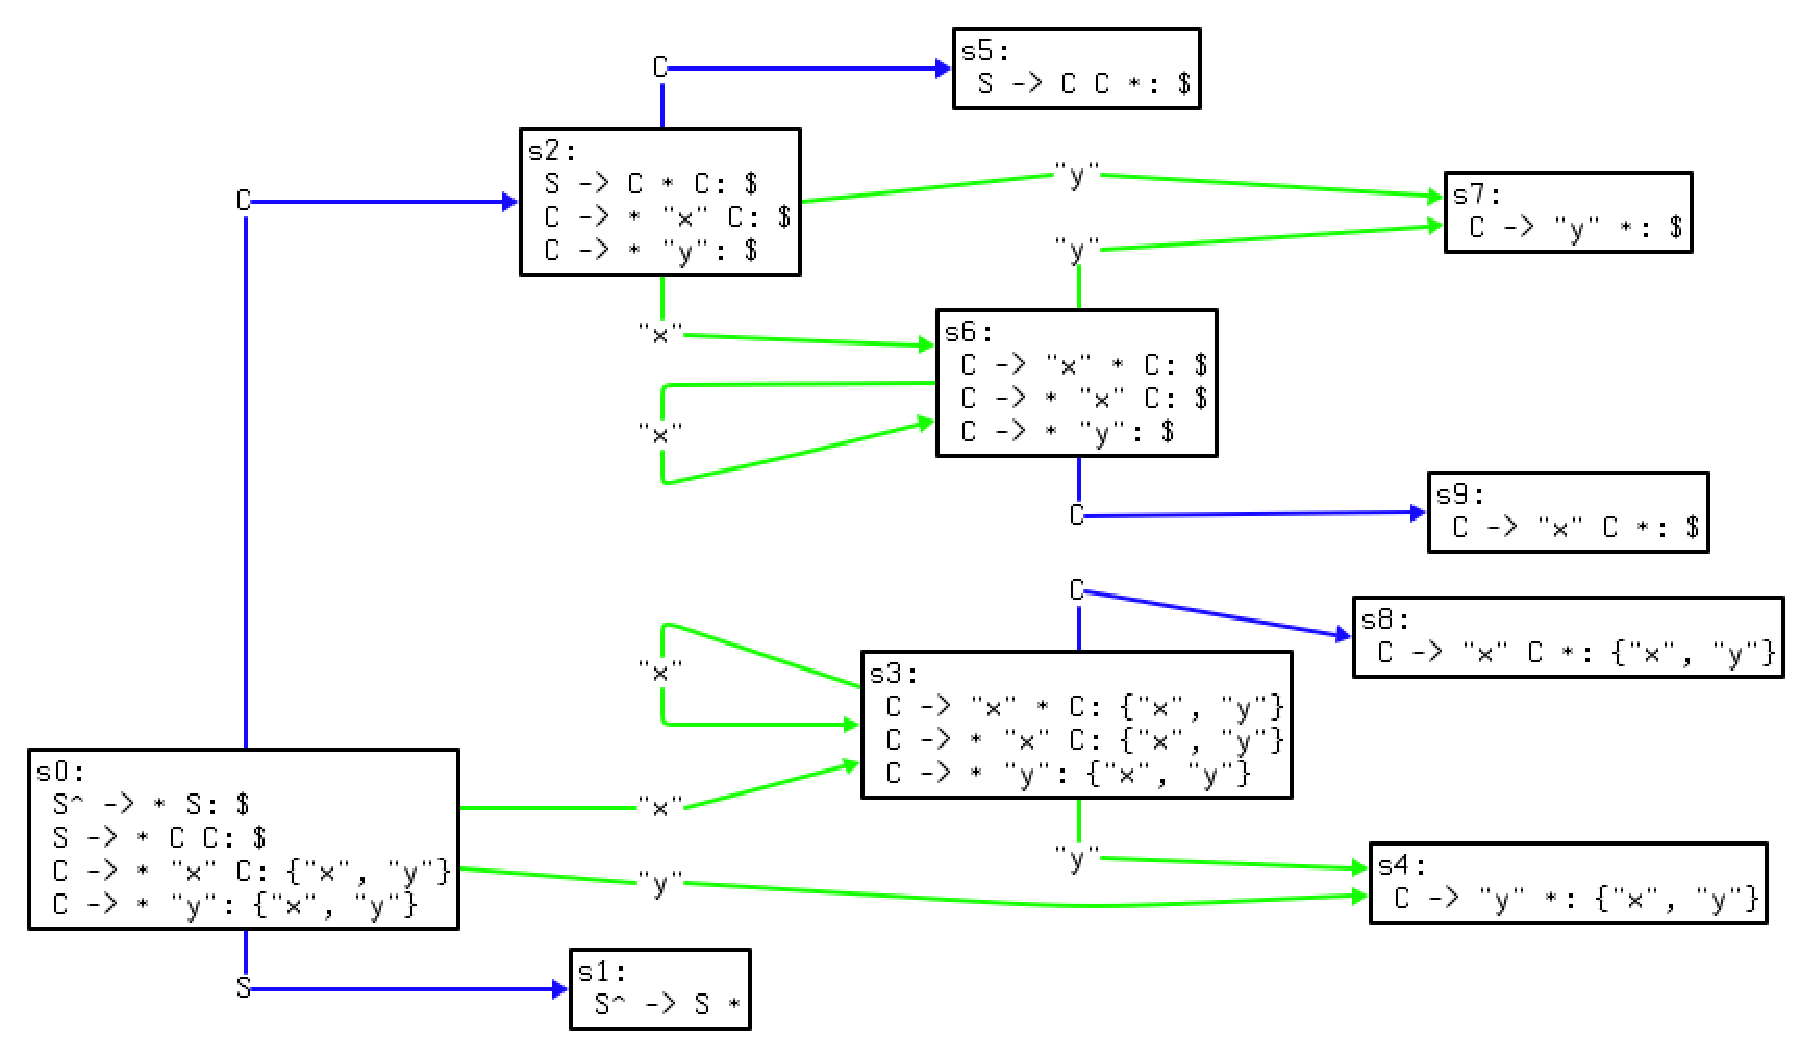
\epsfig{file=../Script/Abbildungen/cc-LR, scale=0.8, angle=90}

\end{slide}

%%%%%%%%%%%%%%%%%%%%%%%%%%%%%%%%%%%%%%%%%%%%%%%%%%%%%%%%%%%%%%%%%%%%%%%%

\begin{slide}{}

\footnotesize
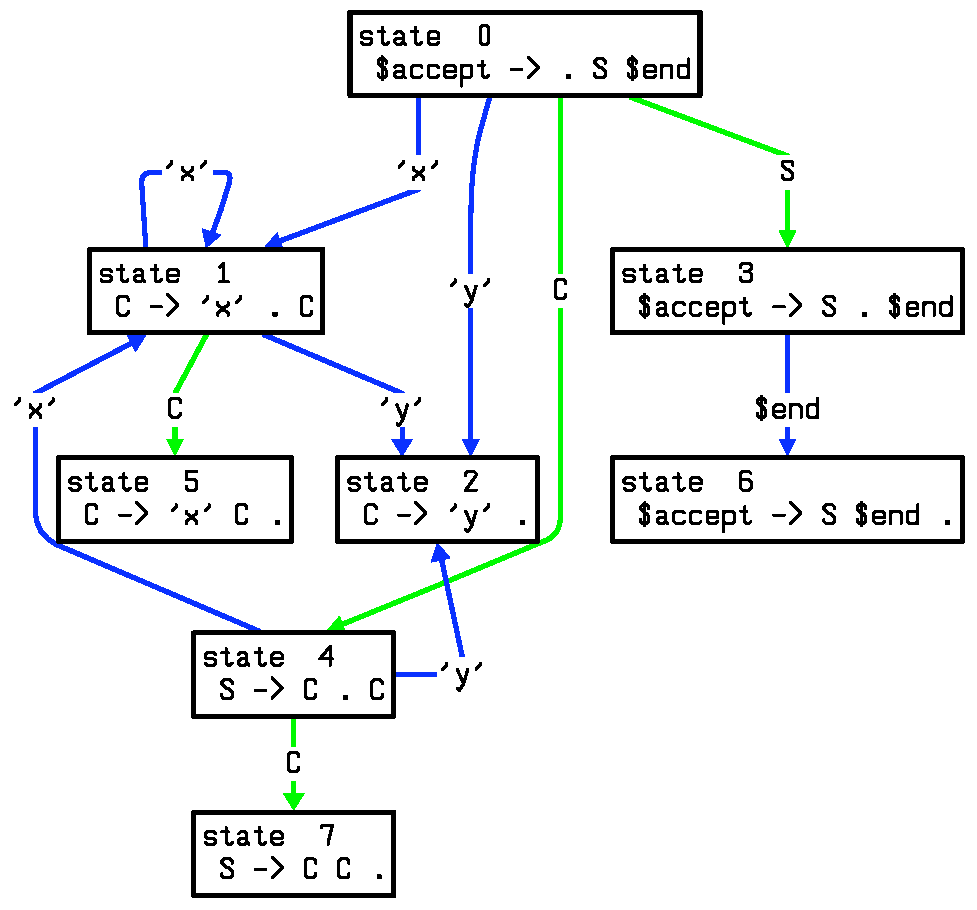
\epsfig{file=../Script/Abbildungen/cc, scale=0.8, angle=90}

\end{slide}
%%%%%%%%%%%%%%%%%%%%%%%%%%%%%%%%%%%%%%%%%%%%%%%%%%%%%%%%%%%%%%%%%%%%%%%%

\begin{slide}{}


  \begin{eqnarray*}    
    \textsl{program}     & \rightarrow & \textsl{typeDefList} \;\; \textsl{signatures}  \;\;\textsl{typedTerms} \\[0.2cm]
    \textsl{typeDefList} & \rightarrow & \textsl{typeDefList}  \;\;\textsl{typeDef} \\[0.0cm]
                         & \mid        & \textsl{typeDef}               \\[0.2cm]
    \textsl{typeDef}     & \rightarrow & \quoted{type} \textsc{Function} \quoted{:=} \textsl{typeSum} \quoted{;} \\[0.0cm]
                         & \mid        & \quoted{type} \textsc{Function} \quoted{(} \textsl{varList} \quoted{)} \quoted{:=} \textsl{typeSum}  \\[0.2cm]    
    \textsl{type}        & \rightarrow & \textsc{Function} \quoted{(} \textsl{typeList} \quoted{)} \\[0.0cm]
                         & \mid        & \textsc{Function}                               \\[0.0cm]
                         & \mid        & \textsc{Variable}                               \\[0.2cm]
    \textsl{typeList}    & \rightarrow & \textsl{typeList} \quoted{,} \textsl{type} \\[0.0cm]
                         & \mid        &  \textsl{type}                     \\[0.2cm]
    \textsl{typeSum}     & \rightarrow & \textsl{typeSum} \quoted{+} \textsl{type} \\[0.0cm]
                         & \mid        & \textsl{type}                   \\[0.2cm]
    \textsl{signature}   & \rightarrow & \quoted{signature} \textsc{Function} \quoted{:} \textsl{argTypes} \quoted{->} \textsl{type} \quoted{;} \\[0.0cm]
                         & \mid        & \quoted{signature} \textsc{Function} \quoted{:} \textsl{type} \quoted{;} \\[0.2cm]
    \textsl{signatures}  & \rightarrow & \textsl{signatures}\;\; \textsl{signature} \\[0.0cm]
                         & \mid        & \textsl{signature}              \\[0.2cm]
    \textsl{argTypes}    & \rightarrow & \textsl{argTypes} \quoted{*} \textsl{type} \\[0.0cm]
                         & \mid        & \textsl{type}                  \\[0.2cm]
    \textsl{varList}     & \rightarrow & \textsl{varList} \quoted{,} \textsc{Variable} \\[0.0cm]
                         & \mid        & \textsc{Variable}                 \\[0.2cm]
    \textsl{term}        & \rightarrow & \textsc{Function} \quoted{(} \textsl{termList} \quoted{)} \\[0.0cm]
                         & \mid        & \textsc{Function}    \\[0.2cm]
    \textsl{termList}    & \rightarrow & \textsl{termList} \quoted{,} \textsl{term} \\[0.0cm]
                         & \mid        & \textsl{term}                  \\[0.2cm]
    \textsl{typedTerm}   & \rightarrow & \textsl{term} \quoted{:} \textsl{type} \quoted{;} \\[0.0cm]    
    \textsl{typedTerms}  & \rightarrow & \textsl{typedTerms}  \;\;\textsl{typedTerm} \\[0.0cm]
                         & \mid        & \textsl{typedTerm}             
  \end{eqnarray*}

\end{slide}

\end{document}

%%% Local Variables: 
%%% mode: latex
%%% TeX-master: t
%%% End: 
